\documentclass[12pt]{standalone}
\usepackage[utf8]{inputenc}
\usepackage[T1]{fontenc}
\usepackage{times}
\usepackage{amsmath,amssymb}
\usepackage[dvipsnames,svgnames]{xcolor}
\usepackage{tikz}
\usetikzlibrary{decorations.pathreplacing, calc, positioning, shapes.geometric, shapes.symbols, arrows.meta, backgrounds, fit, shapes.misc}
\definecolor{RED}{rgb}{1,0,0}
\definecolor{dmrsfill}{HTML}{CDE2FB}
\definecolor{winblue}{HTML}{0D366B}
\definecolor{inksec}{HTML}{52514E}
\begin{document}
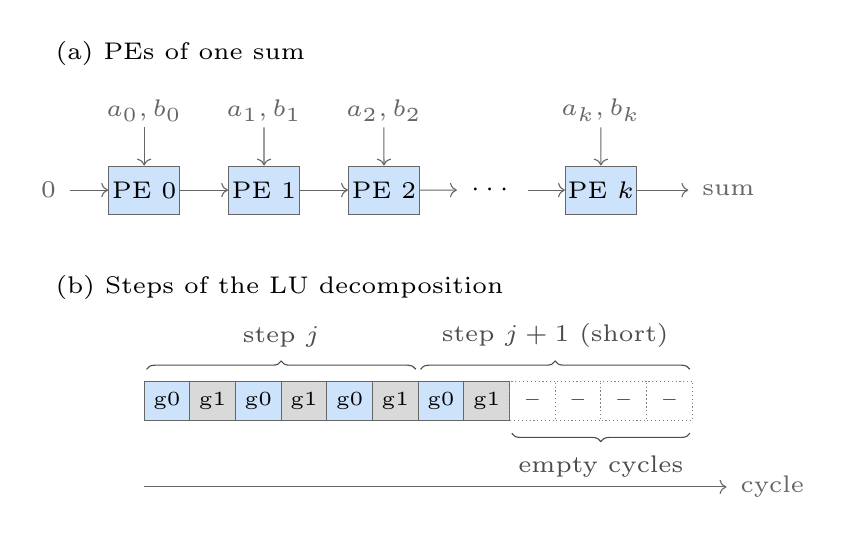
\begin{tikzpicture}[scale=1.45, transform shape, font=\fontsize{6.5}{7.8}\selectfont,
  cel/.style={draw=black!60, fill=#1, minimum width=0.62cm, minimum height=0.42cm, inner sep=0pt, line width=0.3pt},
  cel/.default={white},
  seta/.style={black!60, ->, line width=0.4pt}]
\definecolor{c0}{HTML}{CDE2FB}\definecolor{c1}{HTML}{D9D9D9}
% (a) células em cadeia: s_k = s_{k-1} + a_k b_k
\node[anchor=west] at (-0.9, 1.20) {(a) PEs of one sum};
\foreach \k/\x/\l in {0/0/0, 1/1.05/1, 2/2.10/2} {
  \node[cel=c0] (c\k) at (\x, 0) {PE \l};
  \draw[seta] (\x, 0.55) node[above=-2pt] {$a_{\l}, b_{\l}$} -- (c\k.north);
}
\node (dots) at (3.05, 0) {$\cdots$};
\node[cel=c0] (cn) at (4.0, 0) {PE $k$};
\draw[seta] (4.0, 0.55) node[above=-2pt] {$a_{k}, b_{k}$} -- (cn.north);
\draw[seta] (-0.65, 0) node[left] {$0$} -- (c0.west);
\draw[seta] (c0) -- (c1); \draw[seta] (c1) -- (c2); \draw[seta] (c2) -- (dots); \draw[seta] (dots) -- (cn);
\draw[seta] (cn.east) -- ++(0.45, 0) node[right] {sum};
% (b) passos da LU com ciclos vazios
\begin{scope}[shift={(0,-1.85)}]
\node[anchor=west] at (-0.9, 1.00) {(b) Steps of the LU decomposition};
\def\w{0.40}
\foreach \i/\g in {0/0, 1/1, 2/0, 3/1, 4/0, 5/1} {
  \ifnum\g=0 \def\cc{c0}\else\def\cc{c1}\fi
  \node[cel=\cc, minimum width=0.40cm, minimum height=0.34cm] at (\i*\w+0.5*\w, 0) {\fontsize{5}{6}\selectfont g\g};
}
\foreach \i/\g in {6/0, 7/1} {
  \ifnum\g=0 \def\cc{c0}\else\def\cc{c1}\fi
  \node[cel=\cc, minimum width=0.40cm, minimum height=0.34cm] at (\i*\w+0.5*\w, 0) {\fontsize{5}{6}\selectfont g\g};
}
\foreach \i in {8,...,11}
  \node[draw=black!50, fill=white, densely dotted, minimum width=0.40cm, minimum height=0.34cm, inner sep=0pt, line width=0.4pt] at (\i*\w+0.5*\w, 0) {\fontsize{5}{6}\selectfont --};
\draw[decorate, decoration={brace, amplitude=3pt}, black!70, line width=0.4pt] (0.02, 0.28) -- (6*\w-0.02, 0.28) node[midway, above=2pt] {step $j$};
\draw[decorate, decoration={brace, amplitude=3pt}, black!70, line width=0.4pt] (6*\w+0.02, 0.28) -- (12*\w-0.02, 0.28) node[midway, above=2pt] {step $j+1$ (short)};
\draw[decorate, decoration={brace, mirror, amplitude=3pt}, black!70, line width=0.4pt] (8*\w+0.02, -0.28) -- (12*\w-0.02, -0.28) node[midway, below=2pt] {empty cycles};
\draw[black!60, ->, line width=0.4pt] (0,-0.75) -- (12*\w+0.3,-0.75) node[right] {cycle};
\end{scope}
\end{tikzpicture}
\end{document}
